\paragraph{Как выглядит мейн функция} - вы можете найти на гитхабе в референсах.
Она слишком длинная, чтобы записывать ее в репорт

\paragraph{Описание}

Данный код --- это функция на языке C, которая реализует проверку флага, аналогичную предыдущей, но с поэтапной посимвольной проверкой.
Опишем её по шагам:

\begin{enumerate}
    \item Объявление локальных переменных и инициализация:
    \begin{verbatim}
    int iVar1;
    int local_40;
    int local_3c;
    char local_38 [4];
    char cStack_34;
    char cStack_33;
    ...
    char acStack_13 [7];
    undefined4 local_c;

    local_c = 0;
    local_3c = 0;
    \end{verbatim}

    \item Приветственное сообщение:
    \begin{verbatim}
    printf("%s",
      "Hello, this task is very similar to the
      previous one, but has  some
      modifications\nenter the flag:\n"
    );
    \end{verbatim}
    Выводит сообщение с просьбой ввести флаг.

    \item Чтение посимвольного ввода (38 символов):
    \begin{verbatim}
    for (local_40 = 0; local_40 < 0x26; local_40 = local_40 + 1) {
      __isoc99_scanf(&DAT_00102069, local_38 + local_40);
    }
    \end{verbatim}

    \item Пошаговое посимвольное сравнение (каждый символ сравнивается отдельно через \texttt{strncmp}), например:
    \begin{verbatim}
    iVar1 = strncmp("f", local_38, 1);
    if (iVar1 == 0) {
      local_3c = 1;
      iVar1 = strncmp("l", local_38 + 1, 1);
      if (iVar1 == 0) {
        local_3c = 2;
        iVar1 = strncmp("a", local_38 + 2, 1);
        if (iVar1 == 0) {
          local_3c = 3;
          ...
    \end{verbatim}

    Проверка продолжается символ за символом:
    \begin{verbatim}
    ...
    iVar1 = strncmp("}", acStack_13, 1);
    if (iVar1 == 0) {
      local_3c = 0x26;
    }
    \end{verbatim}

    \item Финальная проверка:
    \begin{verbatim}
    if (local_3c == 0x26) {
      printf("%s", &DAT_00102097);
    }
    else {
      printf("%s", "TRY HARDER");
    }
    \end{verbatim}

    \item Возврат из функции:
    \begin{verbatim}
    return 0;
    \end{verbatim}
\end{enumerate}

\paragraph{Отличия и особенности}
\begin{itemize}
    \item task\_0 считывает строчку - после enter или пробела запустится скрипт дальше, в то время как в task\_1 используется посимвольный ввод

    \item Поскольку флаг состоит из 38 символов, функция будет ждать, пока пользователь не введет 38 символов и только потом запустит дальше

    \item В task\_1 последовательное, посимвольное сравнение с буквами из правильного флага

    \item Флаг для этой задачи немного другой - flag\{444Y0urB4seRBe803g2Usdfd4ds9y1re\}
\end{itemize}

\paragraph{Тестовые запуски}

\paragraph{}

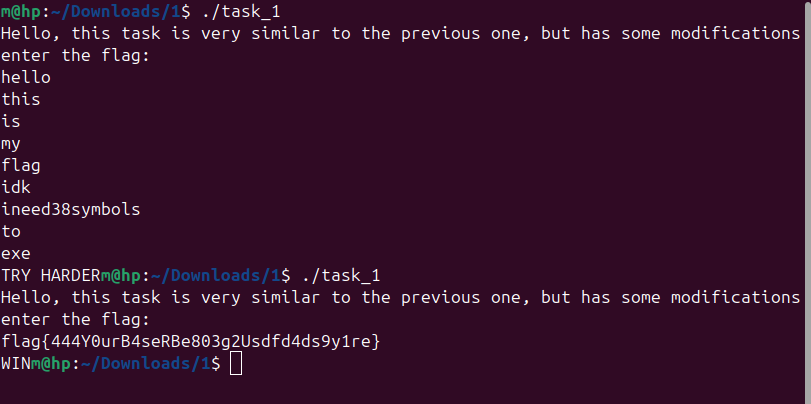
\includegraphics[width=0.75\linewidth]{static/solution_task_1}
